\PassOptionsToPackage{unicode=true}{hyperref} % options for packages loaded elsewhere
\PassOptionsToPackage{hyphens}{url}
%
\documentclass[
  english,
  man,floatsintext]{apa6}
\usepackage{lmodern}
\usepackage{amssymb,amsmath}
\usepackage{ifxetex,ifluatex}
\ifnum 0\ifxetex 1\fi\ifluatex 1\fi=0 % if pdftex
  \usepackage[T1]{fontenc}
  \usepackage[utf8]{inputenc}
  \usepackage{textcomp} % provides euro and other symbols
\else % if luatex or xelatex
  \usepackage{unicode-math}
  \defaultfontfeatures{Scale=MatchLowercase}
  \defaultfontfeatures[\rmfamily]{Ligatures=TeX,Scale=1}
\fi
% use upquote if available, for straight quotes in verbatim environments
\IfFileExists{upquote.sty}{\usepackage{upquote}}{}
\IfFileExists{microtype.sty}{% use microtype if available
  \usepackage[]{microtype}
  \UseMicrotypeSet[protrusion]{basicmath} % disable protrusion for tt fonts
}{}
\makeatletter
\@ifundefined{KOMAClassName}{% if non-KOMA class
  \IfFileExists{parskip.sty}{%
    \usepackage{parskip}
  }{% else
    \setlength{\parindent}{0pt}
    \setlength{\parskip}{6pt plus 2pt minus 1pt}}
}{% if KOMA class
  \KOMAoptions{parskip=half}}
\makeatother
\usepackage{xcolor}
\IfFileExists{xurl.sty}{\usepackage{xurl}}{} % add URL line breaks if available
\IfFileExists{bookmark.sty}{\usepackage{bookmark}}{\usepackage{hyperref}}
\hypersetup{
  pdftitle={The Efficacy of Second-Eye Cataract Surgery},
  pdfkeywords={keywords},
  pdfborder={0 0 0},
  breaklinks=true}
\urlstyle{same}  % don't use monospace font for urls
\usepackage{graphicx,grffile}
\makeatletter
\def\maxwidth{\ifdim\Gin@nat@width>\linewidth\linewidth\else\Gin@nat@width\fi}
\def\maxheight{\ifdim\Gin@nat@height>\textheight\textheight\else\Gin@nat@height\fi}
\makeatother
% Scale images if necessary, so that they will not overflow the page
% margins by default, and it is still possible to overwrite the defaults
% using explicit options in \includegraphics[width, height, ...]{}
\setkeys{Gin}{width=\maxwidth,height=\maxheight,keepaspectratio}
\setlength{\emergencystretch}{3em}  % prevent overfull lines
\providecommand{\tightlist}{%
  \setlength{\itemsep}{0pt}\setlength{\parskip}{0pt}}
\setcounter{secnumdepth}{-2}

% set default figure placement to htbp
\makeatletter
\def\fps@figure{htbp}
\makeatother

% Manuscript styling
\usepackage{upgreek}
\captionsetup{font=singlespacing,justification=justified}

% Table formatting
\usepackage{longtable}
\usepackage{lscape}
% \usepackage[counterclockwise]{rotating}   % Landscape page setup for large tables
\usepackage{multirow}		% Table styling
\usepackage{tabularx}		% Control Column width
\usepackage[flushleft]{threeparttable}	% Allows for three part tables with a specified notes section
\usepackage{threeparttablex}            % Lets threeparttable work with longtable

% Create new environments so endfloat can handle them
% \newenvironment{ltable}
%   {\begin{landscape}\begin{center}\begin{threeparttable}}
%   {\end{threeparttable}\end{center}\end{landscape}}
\newenvironment{lltable}{\begin{landscape}\begin{center}\begin{ThreePartTable}}{\end{ThreePartTable}\end{center}\end{landscape}}

% Enables adjusting longtable caption width to table width
% Solution found at http://golatex.de/longtable-mit-caption-so-breit-wie-die-tabelle-t15767.html
\makeatletter
\newcommand\LastLTentrywidth{1em}
\newlength\longtablewidth
\setlength{\longtablewidth}{1in}
\newcommand{\getlongtablewidth}{\begingroup \ifcsname LT@\roman{LT@tables}\endcsname \global\longtablewidth=0pt \renewcommand{\LT@entry}[2]{\global\advance\longtablewidth by ##2\relax\gdef\LastLTentrywidth{##2}}\@nameuse{LT@\roman{LT@tables}} \fi \endgroup}

% \setlength{\parindent}{0.5in}
% \setlength{\parskip}{0pt plus 0pt minus 0pt}

% \usepackage{etoolbox}
\makeatletter
\patchcmd{\HyOrg@maketitle}
  {\section{\normalfont\normalsize\abstractname}}
  {\section*{\normalfont\normalsize\abstractname}}
  {}{\typeout{Failed to patch abstract.}}
\makeatother
\shorttitle{The Efficacy of Second-Eye Cataract Surgery}
\author{William E. A. Sheppard\textsuperscript{1}, Mary P. Dickerson\textsuperscript{2}, Rigmor Baraas\textsuperscript{3}, Mark Mon-Williams\textsuperscript{1, 4}, Richard M. Wilkie\textsuperscript{1}, \& Rachel O. Coates\textsuperscript{1}}
\affiliation{
\vspace{0.5cm}
\textsuperscript{1} School of Psychology, University of Leeds, Leeds, West Yorkshire, UK \\\textsuperscript{2} Department of Ophthalmology, York Teaching Hospital NHS Foundation Trust, North Yorkshire, UK\\\textsuperscript{3} Department of Optometry, Radiography and Lighting Design, University of South-Eastern Norway, Kongsberg, Norway\\\textsuperscript{4} Bradford Institute of Health Research, Bradford Teaching Hospital NHS Foundation Trust, West Yorkshire, UK}
\authornote{

Correspondence concerning this article should be addressed to Rachel O. Coates, School of Psychology, University of Leeds, Leeds, LS2 9JT . E-mail: r.o.a.coats@leeds.ac.uk}
\keywords{keywords\newline\indent Word count: X}
\usepackage{lineno}

\linenumbers
\usepackage{csquotes}
\ifnum 0\ifxetex 1\fi=0 % if pdftex or luatex
  \usepackage[shorthands=off,main=english]{babel}
\else % if xetex
  % load polyglossia as late as possible as it *could* call bidi if RTL lang (e.g. Hebrew or Arabic)
  \usepackage{polyglossia}
  \setmainlanguage[]{english}
\fi

\title{The Efficacy of Second-Eye Cataract Surgery}

\date{}

\abstract{
\textbf{Abstract.}
}

\begin{document}
\maketitle

Cataract is a common eye condition that involves the progressive clouding of the crystalline lens.
Cataracts typically present bilaterally and cause deterioration in visual function.
Individuals will typically begin to experience these deficits in high and low light conditions and may struggle to carry out tasks such as driving (NHS, 2017).
It is estimated that 48\% of worldwide blindness is due to untreated cataracts.
While the condition can develop at any age, prevalence is far higher in older populations.
Approximately 40\% of those over 65, and 70\% of over 85-year-olds are currently living with at least one cataract; and prevalence along with rates of cataract-related sight loss stand to increase with our ageing population (Nash, 2013).
The loss of vision experienced by those with cataracts can lead to severe decreases in both physical and mental health (Foss et al., 2006); restricting people's ability to carry out daily tasks and diminishing their quality of life (QoL) (Laidlaw et al., 1998).

Surgery is the only proven treatment for cataracts.
In the majority of cases, cataracts are treated through the surgical removal of the clouded lens, before replacing it with an artificial lens.
Cataract removal is considered to be quick and safe; usually lasting \textless{}40 minutes, and with only 1.5\% of cases experiencing severe sight loss, typically only in those with pre-existing co-pathologies (Day, Donachie, Sparrow, \& Johnston, 2015; Nash, 2013).
Cataract surgery is also considered highly cost-effective, even in those with mild visual impairments, and is associated with improvements in visual acuity (VA), contrast sensitivity (CS) and depth perception as well as improved quality of life, reductions in falls, anxiety and depression (Day et al., 2015; Frampton, Harris, Cooper, Lotery, \& Shepherd, 2014; The Royal College of Ophthalmologists, 2018).

As the population becomes older, fall reduction in older adults is becoming a priority for health care providers.
According to guidelines published in 2017, there is now an estimated 255,000 yearly hospital admissions for fall-related injuries, with fragility fractures now costing the NHS over £4 billion per year (Public Health England, 2017).
Reducing this number is therefore imperative.
A longitudinal cohort study of bilateral cataract patients in Vietnam investigated changes to fall risk following bilateral cataract surgery finding a reduction of 83\% (gia To et al., 2014).
Similar work in the USA compared hip fracture rates in pre -- and post-operative bilateral cataract patients.
Compared to pre-operative individuals, the adjusted odds ratio of hip fracture in the first year after cataract removal was 0.84 (95\% CI 0.83 -- 0.89) (Tseng, Yu, Lum, \& Coleman, 2012).

Fall risk is not the only mortality factor reduced by bilateral cataract removal.
When comparing motor crash rates in vehicles driven by pre-operative individuals to those driven by post-operative individuals, longitudinal cohort studies have estimated a crash risk reduction of between 9 -- 13\% with a cost reduction of approx.
\$(AUS)4.3 million (Meuleners, Hendrie, Lee, Ng, \& Morlet, 2012; Schlenker, Thiruchelvam, \& Redelmeier, 2018).
Cost savings were estimated in terms of crash-related medical expenses, loss of income, property damage and other factors.
Cataract surgery is associated with both functional improvements and health indices associated with longevity, such as improved sleep quality and increased gait speed.
By comparing changes in gait speed between the preoperative period to 6-months post-operative (approx. 0.1 ms-1) to standardised longevity-gait speed curves the authors estimated men could expect an increase in life expectancy of 1.5 years and women 1.0 years following bilateral cataract removal (Ayaki, Muramatsu, Negishi, \& Tsubota, 2013; Ayaki, Negishi, \& Tsubota, 2014).

Due to the prevalence of cataracts, elective cataract surgery is the most commonly performed surgical procedure in the NHS.
NICE guidelines published in October 2017 suggested that approximately 400,000 cataract removal surgeries are now performed in the UK each year, at a cost exceeding £290,000,000 (National Institute for Health and Care Excellence, 2017; NHS Improvement, 2017), and rates are only anticipated to rise with increasing life expectancy and a growing population.
The point at which surgery should be performed is a matter of debate, with some Clinical Commissioning Groups (CCGs) introducing a \enquote{managed access} approach based on visual thresholds (Appleby, Devlin, Parkin, Buxton, \& Chalkidou, 2009).
In 2012 it emerged that almost half of commissioners restricted access to cataract surgery by the application of clinical thresholds, and 9 in every 10 cataract surgery commissioners used criteria that reflected neither research evidence nor clinical guidance (Coronini-Cronberg, Lee, Darzi, \& Smith, 2012)

Historically, the threshold at which cataract considered to be \enquote{causing visual impairment} and surgical intervention was offered was defined as VA in one or both eyes poorer than 6/12 (due to lens opacity).
This level is no longer considered an appropriate threshold for surgical intervention.
This is due to higher levels of visual function needed to maintain independence, rising patient expectations, advances in surgical technique, and a disregard of the effect of other symptoms including the effects of glare or reduced CS.
Recommendations now focus on a \enquote{high-quality care pathway}, a patient-centred approach focussed on the needs of the individual.
However, this flexible approach lends itself to subjectivity and variation in decisions made.
Indeed, The Royal College of Ophthalmologists was asked to commission guidelines in 2018 in response to continuing evidence for wide geographical variation across England in access to surgery (The Royal College of Ophthalmologists, 2018) despite current National Institute of Health and Care Excellence (NICE) guidelines stating that arbitrary thresholds of VA should not be used to restrict access to cataract surgery (National Institute for Health and Care Excellence, 2017).

Surgical restrictions (\enquote{managed access}) based on arbitrary thresholds are particularly prevalent for second eye surgery (SES).
Regarding bilateral cataracts, the patient's eye with the worst vision is typically operated on first, with SES then performed after a short delay (Frampton et al., 2014).
Despite the cost reduction associated with immediate sequential bilateral cataract removal these procedures are not routinely carried out due to the fear of serious complications.
These include post-operative infection, endophthalmitis, and poorer refractive outcomes (Lansingh, Eckert, \& Strauss, 2015).
SES is thought to account for approximately 30\% of all cataract removals carried out by the NHS each year (Lundström, Barry, Henry, Rosen, \& Stenevi, 2012).
However, the number of patients receiving SES ranges from 21 -- 58\% across CCGs (RNIB, 2017), meaning patients face a \enquote{postcode lottery}.
This SES restriction exists despite the aforementioned positive outcomes and long-term financial justification of surgery.
There are several factors presumably driving this approach.
Firstly, at least in part, it represents a solution to the growing costs of surgery, and secondly, it is likely to be due to a dearth of information about additional benefits of SES beyond that of single cataract removal.
There is, therefore, an urgent and increasing need for research evaluating the visual and functional benefits of SES.

Since this practice was introduced researchers have attempted have to quantify the clinical and cost-effectiveness of SES.
For example, Cooper and colleagues (2015) aimed to model the average cost of quality-adjusted life years (QALY) gained by binocular cataract patients who received first-eye surgery (FES) followed by SES compared to those who only received FES.
Their model suggested that on average SES generated an additional 0.68 QALY at £1,964 per year, which is far below the thresholds that people would typically be willing to pay (£10,000 - 20,000).
Despite this, the authors go on to state that economic analysis should not be the single motivating factor driving decision making regarding these procedures.
Suggesting that a major limiting factor in the predictive power of their model was a lack of high-quality, modern clinical trials which had collected data on baseline clinical measures such as VA and stereopsis i.e.~an individual's ability to integrate images from both eyes into a single coherent picture of the world facilitating depth perception (Levi, Knill, \& Bavelier, 2015).

The potential benefits of improved visual-motor capabilities following SES are well illustrated in a longitudinal cohort study of over 55s.
Researchers compared fall rates at three time points, before surgery, following FES, and following SES.
Fall rates were found to fall by 54\% following FES compared to pre-surgical levels, but this number increased to 73\% following SES.
Researchers attributed these improvements to improved binocular VA and CS, both of which were correlated with reduced fall risk (Feng, Meuleners, Fraser, Brameld, \& Agramunt, 2018).
When considered together, evidence of functional benefits and the improved quality of life associated with bilateral cataract removal (Levi et al., 2015), demonstrate some advantage of SES over FES alone.
But to best understand this, the underlying visual-motor mechanisms must be further investigated.

Improvements to sight following SES can largely be understood by comparing binocular and monocular vision (Cooper et al., 2015).
These benefits can be seen in both VA (Heravian, Jenkins, \& Douthwaite, 1990) and CS (Baker, Meese, and Hess, 2008), an individual's ability to detect low levels of contrast (Mäntyjärvi \& Laitinen, 2001).
However these advantages tend to be small, for example, Heravian and colleagues (1990) found an average binocular advantage of 1 -- 11\% for VA.
This small effect suggests that the binocular advantage is largely driven by aspects of vision that can only be achieved with two-eyes, such as stereopsis (Jones \& Lee, 1981).
Similar advantages have been found when comparing SES patients to FES only patients.
A systematic review carried out by Frampton and colleagues (2014) compared visual performance in 705 participants who were either waiting for SES to those who had bilateral cataract removal.
Following SES, small insignificant improvements were observed in VA and CS compared to larger, significant improvements to stereopsis.

However, despite the evidence for the clear visual benefits of monocular over binocular vision, when considering performance on motor tasks, the evidence is mixed and largely task-dependent.
For example, Piano and O'Connor (2013) tested 80 18-40-year-olds' ability to complete water pouring and two levels of bead threading tasks (large and small beads).
VA was sequentially reduced across four levels in the participants' non-dominant eye using a convex spherical lens from baseline to suppression.
No significant difference was found across visual conditions in the water pouring (easiest) task.
When comparing task performance time under baseline VA conditions to immeasurably poor VA conditions; the large bad task saw a 37\% increase and the small bead task saw a 42\% increase in task performance time.
Performance deficits were not just observed between baseline and suppression: even at the lowest level of monocular visual distortion (0.5 ± 0.14 logMAR units), significant increases in task performance times were seen in both the large and small bead tasks.

This work by Piano and O'Connor (2013) highlights two of the key floors in vision research that must be addressed going forward.
Firstly, unmeasured visual deficits may produce significant changes to results if they are not accounted for, and secondly, fine motor performance is highly sensitive to task difficulty, highlighting the need for objective and validated tasks.
One such measure is the Clinical Kinematic Assessment Tool (C-KAT) (Culmer, Levesley, Mon-Williams, \& Williams, 2009a); C-KAT consists of a 10-15-minute, tablet-based measure of fine motor skill.
The battery consists of three tasks, tracking, aiming and steering, to be completed in this order.
C-KAT has been repeatedly shown to be able to show differences in fine motor ability such as between participants dominant and non-dominant hands in Culmer and colleagues (2009) original paper and to indicate that prepubescent girls have a small advantage in terms of motor control when compared to their male peers (Flatters, Hill, Williams, Barber, \& Mon-Williams, 2014).
Furthermore, performance in the modified version of the C-KAT steering task has been shown to correlate with VA, providing further evidence of the link between clarity of sight and fine motor skill (Domkin, Richter, Zetterlund, \& Lundqvist, 2016).

\emph{This study.}

To address the issues outlined above the present study will consist of two experiments.
Firstly, an experiment comparing performance on a fine motor skill battery under binocular and monocular (better visual acuity eye and worse visual acuity eye) visual conditions.
Secondly, an experiment investigating how vision and visual-motor performance are affected by simulated cataracts.
This experiment will be carried out under three conditions: clear binocular vision, unilateral simulated cataract and bilateral simulated cataracts.
Together these experiments will hope to disentangle the benefits of SES over FES alone.

\hypertarget{experiment-1.-monocular-versus-binocular-vision}{%
\section{Experiment 1. Monocular versus binocular vision}\label{experiment-1.-monocular-versus-binocular-vision}}

\hypertarget{methods}{%
\section{Methods}\label{methods}}

\hypertarget{participants}{%
\subsection{Participants}\label{participants}}

74 undergraduate students (19 males) from the University of Leeds participated in the present study and were recruited by opportunity sampling.
Two participants had to be removed as they did not complete the Binocular condition, leaving an n of 72.
Participants were aged 19 -- 24 years old (mean = 20.3, SD = 1.8).
Seven participants were left-handed, 14 had corrected-to-normal vision (glasses or contact lenses).
No participants reported any history of tremors or impaired motor function that might affect their ability to perform the tasks.
Participants were not compensated for their participation.
Ethical approval was granted by the University of Leeds Research Ethics Committee (Ethics Reference Number: 15-0264).

\hypertarget{materials}{%
\subsection{Materials}\label{materials}}

Fine motor control was measured using the Clinical Kinematic Assessment Tool: a tool that provides objective measures of sensorimotor performance (Culmer et al., 2009b).
C-KAT presents interactive visual stimuli on a tablet laptop screen whilst recording participants' kinematic responses to these stimuli.
The CKAT was presented on Toshiba portable tablet computers (Portege M700-13P, screen size = 303x190mm, resolution = 1280x800).
A pen-shaped stylus (140 x 9 mm) was used as the input device.
The three CKAT tasks were presented on the tablet screen in landscape orientation on a level table in front of the participant.
The CKAT software records stylus position to capture various kinematic measures (e.g.~movement time, peak speed) to provide information about the accuracy and efficiency of participants' movements.
For a full overview of the CKAT software and tests see (Culmer et al., 2009b; Flatters et al., 2014).

VA was measured using a by the LogMAR standardized test (Bailey and Lovey, 1976).
This chart consisted of 14 rows each with five letters equally distanced from each other and of identical legibility (Siderov \& Tiu, 1999).
Participants stood 6m from the chart and were instructed to sequentially read the letters from each row until the letters became too small for them to read.
A VA score was calculated for each visual condition from the number of letters correctly identified.
A low score demonstrated good VA. VA scores were used to identify the \enquote{better eye} for each participant.

\hypertarget{procedure}{%
\subsection{Procedure}\label{procedure}}

Upon arrival, participants were presented with an information sheet, consent was given and demographic, handedness and vision (corrected/uncorrected) information was recorded.
Each participant then completed the LogMAR eye test and then the CKAT under three vison conditions (left eye, right eye, and both eyes).
Order of vision conditions was counterbalanced. For the monocular conditions (left or right eye) a blindfold was used to cover the eye not being tested.

\hypertarget{the-sensorimotor-battery}{%
\subsubsection{The sensorimotor battery}\label{the-sensorimotor-battery}}

This battery contains three tasks (tracking, aiming and steering), lasting approximately 12-15 minutes in total. Figure 1 shows a graphical representation of the tasks.
\textbf{Insert CKAT diagram and caption here}

\hypertarget{tracking.}{%
\subsubsection{Tracking.}\label{tracking.}}

Participants were required to keep the stylus within the area of a green circle moving in a \enquote{figure-of-8} around the screen.
The circle completed nine revolutions of the screen getting faster every three revolutions.
This task consisted of two trials, the first was unguided, and the second was guided.
In the guided condition a \enquote{figure-of-8} guide was visible on the screen.
Trials lasted approx. 63s each.
Mean RMSE was calculated for each speed and guide condition, whereby a lower score indicated better performance.

\hypertarget{aiming.}{%
\subsubsection{Aiming.}\label{aiming.}}

Participants were required to keep the stylus in constant contact with the screen while moving it as quickly as possible from the start position to a green dot on the screen.
Upon reaching the dot it would disappear and a new dot would appear elsewhere on the screen, which the participant would then move to. All targets were equidistant.
The participant made a total of 75 movements taking approx. 2-4 minutes.
The time taken from arrival at sequential dots, movement time (MT) was recorded.
The median MT for the first 50 movements is reported here, with lower scores indicative of better performance.

\hypertarget{steering.}{%
\subsubsection{Steering.}\label{steering.}}

Participants began the task by touching the tip of the stylus in the 'Start' position. Participants were then presented with a standard pathway made from two parallel lines.
The pathway contained both straights and curves.
The participants were required to move the stylus from the \enquote{Start} to the \enquote{Finish} position without removing the stylus from the screen.
Speed was controlled using a \enquote{pacing box}.
This was a box overlaid on the track that participants were instructed to stay within.
The box moved every 5 seconds. participants completed two trials, both using the same track, but it was reversed for the second trial, each trial took approx. 40 seconds.
The difference between the stylus position and the ideal path, path accuracy (PA, mm), was recorded.
A second measure, penalised path accuracy (pPA, mm) was also calculated as: pPA = Path Accuracy * (1+((Movement time - 36)/36)).
This penalised participants for times when they did not remain within the 'pacing box'.

\hypertarget{design}{%
\subsection{Design}\label{design}}

A repeated measures design was used, with visual condition (Better Eye, Worse Eye, Binocular) as the independent variable for all measures (tracking, aiming and steering).
The statistical software package JASP was used to conduct repeated measures ANOVAs to examine differences between each level of visual condition.
For tracking, an additional two independent variables were factored into a 3x3x2 (visual condition x speed x guide) repeated measures ANOVA.
Where Mauchly's test of sphericity was violated, a Greenhouse-Geisser correction was applied.
Pairwise comparisons were used to explore significant main effects, and a Bonferroni Holm correction was applied.
The only interaction that emerged in the tracking task did not include visual condition (our primary variable of interest) so we did not unpack it with further tests due to the focus of this paper.
We first ran analyses with all participants included, and then reran them excluding those with a logMAR score over \textgreater{}0.2 in either eye to determine whether patterns remained when only participants with reasonably good VA were included.
For reasons of brevity, we only report the statistics for the second set of analyses when the overall findings differ.
\textbf{Insert design figure here}

\hypertarget{results}{%
\section{Results}\label{results}}

\hypertarget{tracking}{%
\subsection{Tracking}\label{tracking}}

One participant had to be removed as they failed to complete the tracking task using their worse eye only due to a technical failure leaving an N of 71.
No main effect of visual condition emerged, F(1.65, 115.68) = 1.44, p =.24, \(\eta^2\) = .02.
There were significant main effects for guide, F(1,70) = 5.29, p \textless{}.02, \(\eta^2\) = .07, and speed, F(1.04,72.59) = 235.21, p \textless{}.001, \(\eta^2\) = .77, and a guide by speed interaction, F(1.07,74.65) = 10.10, p \textless{}.01, \(\eta^2\) = .13 but no interactions involving visual condition.
This pattern of results was the same when all participants with a logMAR score over \textgreater{}0.2 in either eye were excluded (remaining n=55).

\begin{figure}

{\centering 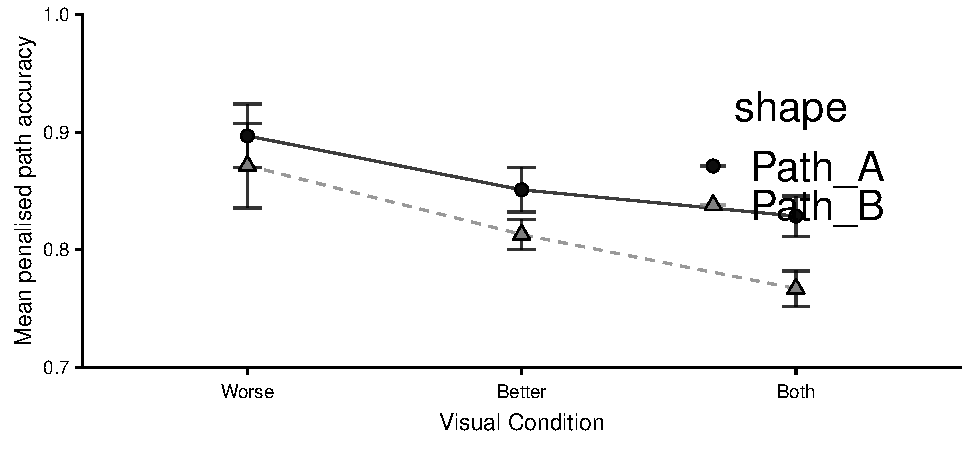
\includegraphics{cataracts_paper_giveup_files/figure-latex/unnamed-chunk-1-1} 

}

\caption{ }\label{fig:unnamed-chunk-1}
\end{figure}

\hypertarget{aiming}{%
\subsection{Aiming}\label{aiming}}

Aiming scores were highest/worst in the worse eye condition and lowest/best in the binocular condition (better eye mean(SD) = 1.12(.16), worse eye mean(SD) = 1.13(.14), binocular mean = 1.05(.14)).
A significant main effect of visual condition emerged F(2,142) = 12.61, p \textless{}.01, \(\eta H\) \(\eta^2\) = .15.
This was driven by significant differences in aiming scores between binocular vision and the better eye, p \textless{}.001, \emph{Cohen's d} = .46, binocular vision and the worse eye, p \textless{}.001, \emph{Cohen's d} = .56 but not between the two monocular conditions, p = .48, \emph{Cohen's d} = .08.
As with tracking, this pattern of results was the same when all participants with a logMAR score over \textgreater{}0.2 in either eye were excluded (remaining N = 56).

\begin{figure}

{\centering 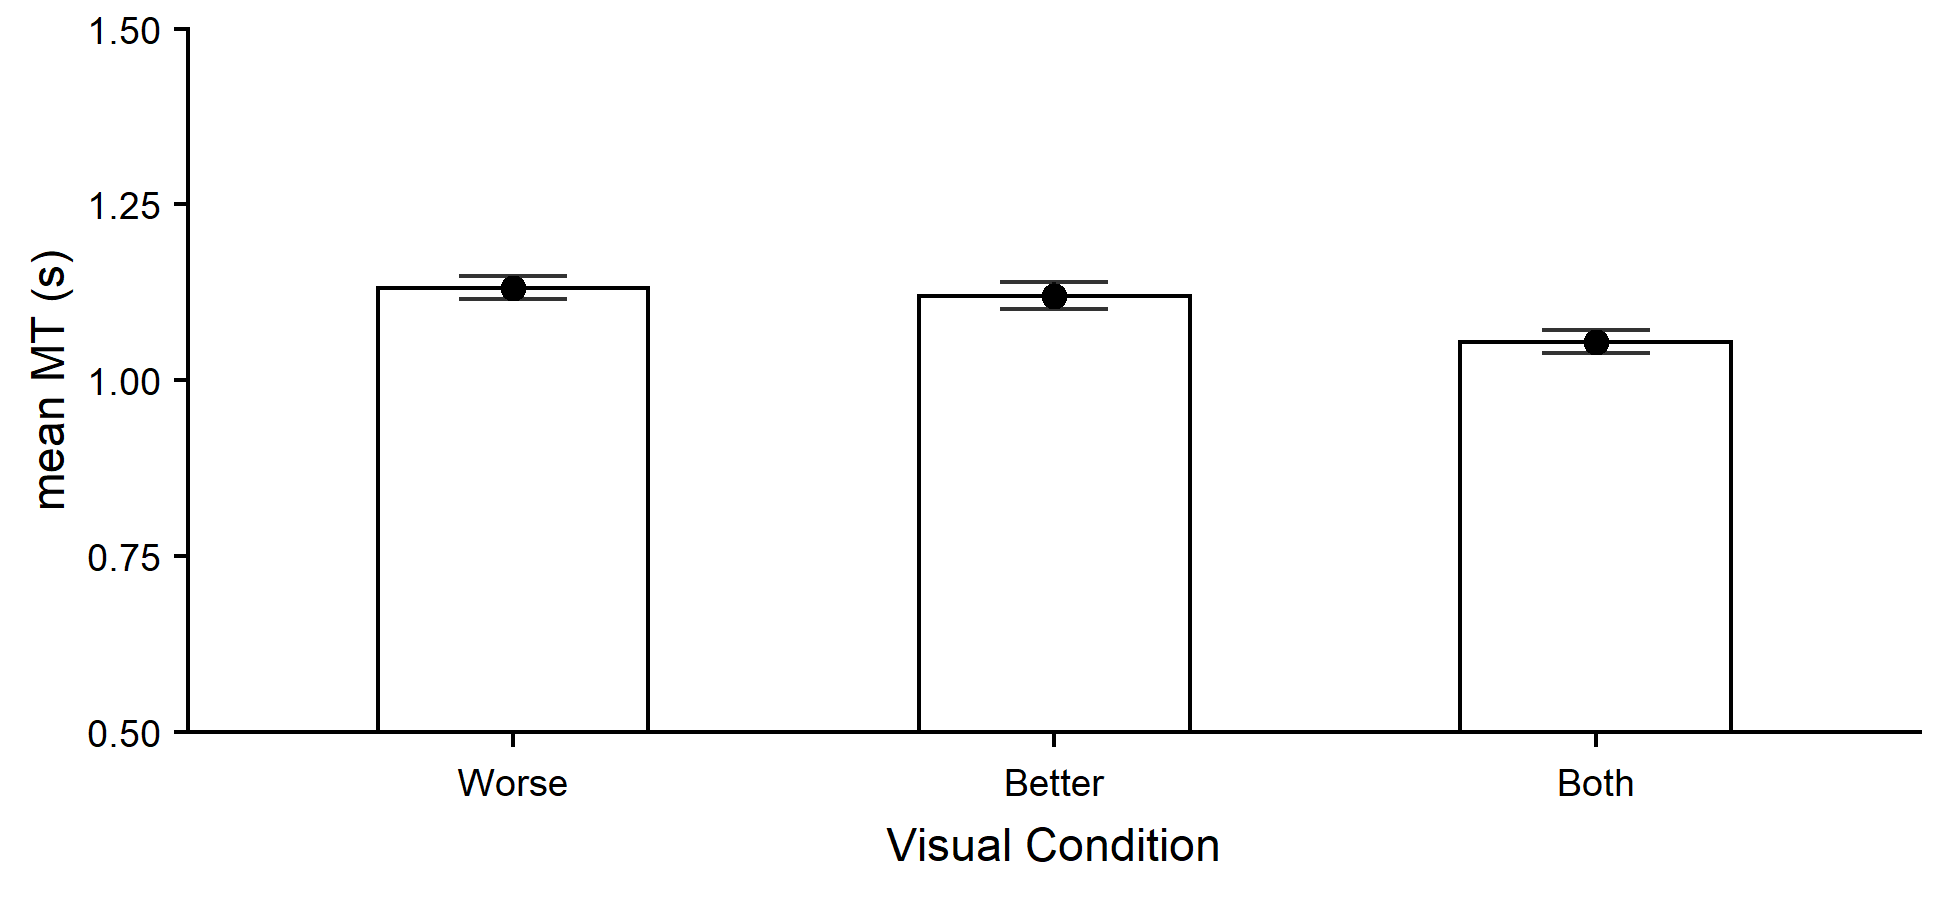
\includegraphics{cataracts_paper_giveup_files/figure-latex/unnamed-chunk-2-1} 

}

\caption{ }\label{fig:unnamed-chunk-2}
\end{figure}

\hypertarget{steering}{%
\subsection{Steering}\label{steering}}

Steering pPA scores were highest/worst in the worse eye condition and lowest/best in the binocular condition (Shape A: better eye mean(SD) = .85(.16), worse eye mean(SD) = .90(.23), binocular mean = .83(.14)) (Shape B: better eye mean(SD) = .81(.11), worse eye mean(SD) = .87(.31), binocular mean = .77(.13)).
A significant main effect of visual condition emerged F(1.38,97.77) = 8.94, p \textless{}.001, \(\eta^2\) = .11.
This was driven by significant differences in aiming scores between binocular vision and the better eye, p \textless{}.05, \emph{Cohen's d} = .34, binocular vision and the worse eye, p \textless{}.001, \emph{Cohen's d} = .44 and between the two monocular conditions, p \textless{}.05, \emph{Cohen's d} = .25.
A main effect of shape emerged, F(1,71) = 8.16, p \textless{}.01, \(\eta^2\) = .10.

This pattern of results was slightly different after excluding all participants with a logMAR score \textgreater{}0.2 in either eye (remaining n=56).
The main effect of shape became not significant, F(1,55) = 3.74, p =.058, \(\eta^2\) = .06.
The main effect of visual condition remained F(1.37,75.07) = 4.66, p \textless{}.05, \(\eta^2\) = .08, but this was now only driven by a significant difference between binocular vision and the worse eye, p \textless{}.05, \emph{Cohen's d} = .37.
There was no difference between binocular vision and the better eye, p =.08, \emph{Cohen's d} = .28 or between the two monocular conditions, p =.13, \emph{Cohen's d} = .20.

\begin{figure}

{\centering 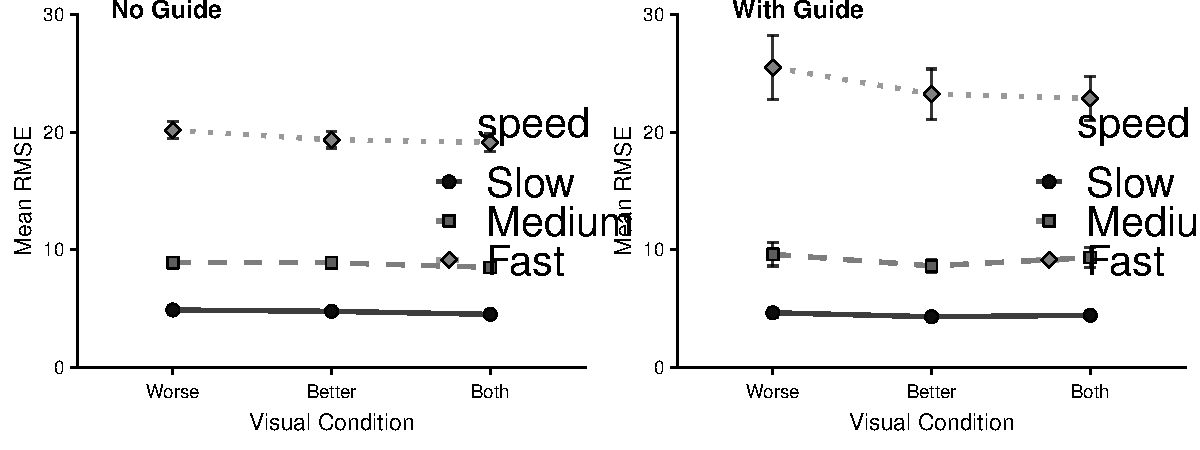
\includegraphics{cataracts_paper_giveup_files/figure-latex/unnamed-chunk-3-1} 

}

\caption{ }\label{fig:unnamed-chunk-3}
\end{figure}

\hypertarget{discussion}{%
\section{Discussion}\label{discussion}}

The present study aimed to investigate whether performance on a fine motor task: tracking, aiming and steering tasks from the C-KAT battery, was significantly better when using two eyes compared to one and whether this was affected when using their \enquote{better} eye compared to their \enquote{worse} eye.
With regards to tracking, performance was significantly better with a guide than without and participants more accurately traced the target at lower speeds.
However, there was no main effect of visual condition, suggesting that monocular vision is sufficient for tracking a moving object, and this was regardless of VA.
In the aiming task, a main effect of visual condition was found showing a binocular advantage over both monocular conditions but no difference was found between the two monocular conditions (\enquote{better} eye, \enquote{worse} eye).
A binocular advantage was also found in the steering task, however, an advantage of the \enquote{better} eye was now also seen over the \enquote{worse} eye.
When excluding participants with the worst vision differences were no longer evident between binocular and \enquote{better} eye conditions, or between the two monocular conditions.

These findings generally demonstrate the benefit of binocular advantage in a 2D fine motor task.
Stereo-reduction is not only seen in individuals with binocular disparities such as those with amblyopia.
In a review of the effect of amblyopia on everyday tasks, Grant and Moseley (2011) noted that amblyopes not only struggle with 3D tasks such as water pouring and bead threading but also struggle with 2D tracing and handwriting tasks.
They go on to report that the deficits associated with the condition become larger with increased task difficulty and novelty and can have life-altering effects by impairing the patient's ability to drive, read and sometimes walk.
Alongside the results of the present study, this provides a compelling rationale to investigate the disparities in visuomotor performance under conditions of normal binocular vision, unilateral and bilateral cataracts.

\hypertarget{experiment-2.-simulated-cataracts}{%
\section{Experiment 2. Simulated cataracts}\label{experiment-2.-simulated-cataracts}}

\hypertarget{methods-1}{%
\section{Methods}\label{methods-1}}

\hypertarget{participants-1}{%
\subsection{Participants}\label{participants-1}}

30 undergraduate students (27 females) from the University of Leeds participated in the present study and were recruited by opportunity sampling through the university of Leeds participant pool.
Participants were aged 18 -- 23 (mean = 19.37, SD = 1.22) years old, five participants were left-handed.
Participants were required to be 18 years old or over and have normal or corrected-to-normal vision.
No participants reported any history of tremors or impaired motor or neurological function that might affect their ability to perform the tasks.
Participants received four course credits as compensation for their participation.
Ethical approval was granted by the University of Leeds Research Ethics Committee (Ethics Reference Number: PSC-192).

\hypertarget{materials-1}{%
\subsection{Materials}\label{materials-1}}

Cataracts were simulated using Bangerter foils attached to one or both lenses of non-prescription glasses. Driver and Vehicle Licensing Agency (DVLA) legislation requires a minimum an individual to have a minimum VA of 6/12 to be allowed to legally drive (DVLA, 2018) i.e.~an individual with 6/12 vision would be able to read from a distance of 6m what an individual with \enquote{normal} vision would be able to read at 12m. The present study, therefore, intended to mimic this level of VA for the cataract conditions. However, research by Dickinson and Taylor (2011) has suggested that 6/15 Bangerter foils more accurately mimic 6/12 vision, therefore 6/15 Bangerter foils will be used in the present study.

VA was measured using the LogMAR standardized test (Bailey \& Lovie, 1976) as described in Experiment 1.

Contrast sensitivity was assessed using the standardized Hamilton-Veale Contrast Sensitivity Test (Karali, Mansfield, \& Gyi, 2017).
Participants stood 1m away from a wall-mounted chart (located at eye-height) consisting of consisted of 16 identically spaced and sized pairs of letters over 8 rows, the letters varied in contrast only, ranging from, 0 to 2.25 log units (Bilen, Hepsen, \& Acre, 2016a).
Each pair differed in contrast with an increment of 0.15 log units (Bilen, Hepsen, \& Acre, 2016b).
Participants were instructed to read aloud as many letters as they could.
Each letter read by the participant gave a score of 0.5, therefore the higher the score, the greater the CS.

Stereopsis was assessed using the Wirt Circles test from the standardized Titmus Stereo Fly Test (Fricke \& Siderov, 1997).
Participants were presented with a chart containing nine diamond shapes (three rows of three diamonds, with each diamond containing four circles, one in each corner).
The chart was held 40cm from the participants' eyes and the participant was asked to state which of the four circles appeared to be the closest.
This was performed while wearing a pair of polarised glasses over simulated cataracts.
Due to the polarised glasses, one circle was predicted to appear the closest and was designated the correct answer.
Participants gained a point for each correct answer, therefore a score of nine as the highest score, and zero the lowest.

The Purdue Pegboard is a standardized measure of upper body and fine motor skills (Tiffin, 1968; Tiffin \& Asher, 1948).
Sitting directly in front of the Purdue Pegboard, participants were instructed to use their dominant hand, taking one pin at a time and placing them into the row of holes that corresponded with their dominant hand.
Participants were required to place possible within 30 seconds, starting with the hole furthest away from them.
Participants were instructed to not replace incorrectly placed pins.
The total number of correctly placed pins was recorded, where a high number demonstrated good fine motor skills.

Participants completed the aiming task of the CKAT battery as described in Exp. 1, but with reduced dot contrast to increase the task difficulty.
As per Experiment 1, MT was the measure of performance, whereby low MT was indicative of better fine motor skill.

For water pouring, as used by O'Connor and colleagues (2010), participants were seated 30cm from five horizontally aligned plastic beakers.
Participants were required to fill each jug to a 40ml mark as quickly and accurately as possible using a jug containing 500ml of water.
Participants were not allowed to touch the beakers or to refill a beaker on a second attempt.
Absolute accuracy (the total volume of water either above or below the 40ml marker) and time in seconds were recorded.
Lower scores in both measures were indicative of more accurate and faster water pouring respectively.
A composite measure of water-pouring performance was calculated using multiplication of absolute accuracy and time.
A lower composite score indicated an overall better water-pouring performance.

\hypertarget{procedure-1}{%
\subsection{Procedure}\label{procedure-1}}

After consenting, participants provided demographic, handedness and vision (corrected/uncorrected) information.
All participants completed the tasks in the same order (Purdue Pegboard, CKAT Aiming, Water-pouring), but the order of the visual condition was counterbalanced between participants.

\begin{figure}

{\centering \includegraphics{C:/Users/wills/Documents/Cataract/Figures/Procedure_Diagram} 

}

\caption{ }\label{fig:unnamed-chunk-4}
\end{figure}

\hypertarget{design-1}{%
\subsection{Design}\label{design-1}}

A repeated measures design was used with visual condition (no filters, 1 filter, 2 filters) as the independent variable for all measures.
The statistical software package JASP was used to conduct repeated measures ANOVAs to examine differences between each level of visual condition.
Where Mauchly's test of sphericity was violated, a Greenhouse-Geisser correction was applied.
Pairwise comparisons were used to explore the significant main effects of visual condition, and a Bonferroni Holm correction was applied.

\hypertarget{results-1}{%
\section{Results}\label{results-1}}

\hypertarget{visual-measures.}{%
\subsection{Visual measures.}\label{visual-measures.}}

\hypertarget{visual-acuity.}{%
\subsubsection{Visual acuity.}\label{visual-acuity.}}

VA (logMAR) was worst/highest in the 2 filter condition and best/lowest in the no filter condition (no filter mean(SD) = -.02(.12), 1 filter mean(SD) = .01(.13), 2 filter mean = .33(.11)).
A significant main effect of visual condition emerged, F(2, 58) = 293.37, p \textless{}.001, \(\eta^2\) 2 = .91.
This was driven by significant differences in logMAR scores between no filter and 1 filter, p \textless{}.05, \emph{Cohen's d} = .40, no filter and 2 filters, p \textless{}.001, \emph{Cohen's d} = 3.63 and between 1 filter and 2 filters, p \textless{}.001, \emph{Cohen's d} = 3.51.

\begin{figure}

{\centering \includegraphics{C:/Users/wills/Documents/Cataract/Figures/VisualAcuity_exp2} 

}

\caption{ }\label{fig:unnamed-chunk-5}
\end{figure}

\hypertarget{contrast-sensitivity.}{%
\subsubsection{Contrast Sensitivity.}\label{contrast-sensitivity.}}

CS scores were worst/lowest in the 2 filter condition and best/highest in the no filter condition (no filter mean(SD) = 12.53(.59), 1 filter mean(SD) = 12.12(.41), 2 filter mean = 10.82(.77)).
A significant main effect of visual condition was found F(1.51, 43.75) = 74.49, p \textless{}.001, \(\eta^2\) = 0.72.
This was driven by significant differences in scores between no filter and 1 filter, p \textless{}.001, \emph{Cohen's d} = .79, no filter and 2 filters, p \textless{}.001, \emph{Cohen's d} = 1.87 and between 1 filter and 2 filters, p \textless{}.001, \emph{Cohen's d} = 1.44.

\begin{figure}

{\centering \includegraphics{C:/Users/wills/Documents/Cataract/Figures/ConstrastSensitivity_exp2} 

}

\caption{ }\label{fig:unnamed-chunk-6}
\end{figure}

\hypertarget{stereopsis.}{%
\subsubsection{Stereopsis.}\label{stereopsis.}}

Stereopsis scores were worst/lowest in the 1 filter condition and best/highest in the no filter condition (no filter mean(SD) = 6.43(2.49), 1 filter mean(SD) = 2.93(2.18), 2 filter mean = 3.87(2.01)).
A significant main effect of visual condition emerged, F (1.66, 48.03) = 45.76, p \textless{}.001, \(\eta^2\) = 0.61.
This was driven by significant differences in scores between no filter and 1 filter, p \textless{}.001, \emph{Cohen's d} = 1.40, no filter and 2 filters, p \textless{}.001, \emph{Cohen's d} = 1.45 and between 1 filter and 2 filters, p \textless{}.011, \emph{Cohen's d} = 0.50.

\begin{figure}

{\centering \includegraphics{C:/Users/wills/Documents/Cataract/Figures/Steroacuity_exp2} 

}

\caption{ }\label{fig:unnamed-chunk-7}
\end{figure}

\hypertarget{motor-measures.}{%
\subsection{Motor measures.}\label{motor-measures.}}

\hypertarget{purdue-pegboard.}{%
\subsubsection{Purdue pegboard.}\label{purdue-pegboard.}}

Pegboard scores were best/highest under the no filter condition and worst/lowest in the 2 filters condition (no filter mean(SD) = 15.0(1.72), 1 filter mean(SD) = 14.93(1.72), 2 filter mean = 14.27(1.55)).
A significant main effect of visual condition emerged, F (2, 58) = 4.76, p \textless{}.05, \(\eta^2\) = 0.14.
This was driven by significant differences in scores between no filter and 2 filters, p \textless{}.05, \emph{Cohen's d} = .50 and between 1 filter and 2 filters, p \textless{}.05, \emph{Cohen's d} = 0.47, but not between no filter and 1 filter, p =.80, \emph{Cohen's d} = .05.

\begin{figure}

{\centering \includegraphics{C:/Users/wills/Documents/Cataract/Figures/Pegboard_exp2} 

}

\caption{ }\label{fig:unnamed-chunk-8}
\end{figure}

\hypertarget{aiming.-1}{%
\subsubsection{Aiming.}\label{aiming.-1}}

Aiming scores were best/lowest in the no filter condition and worst/highest in the 2 filter condition (no filter mean(SD) = 1.21(0.32), 1 filter mean(SD) = 1.23(0.25), 2 filter mean = 1.28(0.27)).
No main effect of visual condition emerged F (2, 58) = 0.984, p =.38, \(\eta^2\) = 0.03.\\
However, two participants had mean scores more than two standard deviations away from the group mean, and these were caused by more than 50\% of trials being over 2 seconds in length in the first visual condition they completed (no filter for P13, 1 filter for P16).
If these participants are removed from the analysis (leaving an n of 28) the main effect of visual condition becomes significant.
Aiming scores were best/lowest in the no filter condition and worst/highest in the 2 filter condition (no filter mean(SD) = 1.15(0.19), 1 filter mean(SD) = 1.18(0.18), 2 filter mean = 1.26(0.27)).
A main effect of visual condition emerged F (2, 54) = 4.41, p \textless{}.05, \(\eta^2\) = 0.14. This was driven by significant differences in scores between no filter and 2 filters, p \textless{}.05, \emph{Cohen's d} = .52, but not between no filter and 1 filter, p =.23, \emph{Cohen's d} = .23, or 1 filter and 2 filters, p =.19, \emph{Cohen's d} = 0.33.

\begin{figure}

{\centering \includegraphics{C:/Users/wills/Documents/Cataract/Figures/Aiming_exp2} 

}

\caption{ }\label{fig:unnamed-chunk-9}
\end{figure}

\hypertarget{water-pouring.}{%
\subsubsection{Water-pouring.}\label{water-pouring.}}

Water-pouring time scores were higher in the 1 and 2 filter conditions compared to the no filter condition (no filter mean(SD) = 15.40(2.90), 1 filter mean(SD) = 16.28(4.08), 2 filter mean = 16.03(14.21), but no main effect of visual condition emerged, F (2, 58) = 1.95, p = .152, \(\eta^2\) = 0.06.

\begin{figure}

{\centering \includegraphics{C:/Users/wills/Documents/Cataract/Figures/WaterPouring-Time_exp2} 

}

\caption{ }\label{fig:unnamed-chunk-10}
\end{figure}

For accuracy, participants were most accurate in the no filter condition and least accurate in the 2 filter condition (no filter mean(SD) = 11.30(9.57), 1 filter mean(SD) = 14.80(8.34), 2 filter mean = 18.70(9.43).
A significant main effect of visual condition emerged, F (2, 58) = 5.79, p \textless{}.01, \(\eta^2\) = 0.16.
This was driven by significant differences in scores between no filter and 2 filters, p \textless{}.01, \emph{Cohen's d} = .59 but not between no filter and 1 filter, p =.18, \emph{Cohen's d} = .32, or 1 filter and 2 filters, p =.18, \emph{Cohen's d} = 0.32.

\begin{figure}

{\centering \includegraphics{C:/Users/wills/Documents/Cataract/Figures/WaterPouringAccuracy_exp2} 

}

\caption{ }\label{fig:unnamed-chunk-11}
\end{figure}

Taking both speed and accuracy together, the composite measure of speed\emph{accuracy showed lowest/best scores under the no filter condition and highest/worst scores under the 2 filter condition (no filter mean(SD) = 165(132), 1 filter mean(SD) = 238(145), 2 filter mean = 294(152)).
A main effect of visual condition was found F (2, 58) = 6.70, p \textless{}.01, \(\eta^2\) = 0.19.
This was driven by significant differences in scores between no filter and 1 filter, p =.05, }Cohen's d* = .43 and between no filter and 2 filters, p \textless{}.01, \emph{Cohen's d} = .65 but not between 1 filter and 2 filters, p =.16, \emph{Cohen's d} = 0.27.

\begin{figure}

{\centering \includegraphics{C:/Users/wills/Documents/Cataract/Figures/WaterpouringTimebyaccuracy_exp2} 

}

\caption{ }\label{fig:unnamed-chunk-12}
\end{figure}

\hypertarget{discussion-1}{%
\section{Discussion}\label{discussion-1}}

The present study aimed to assess the impact of SES in a non-clinical population by investigating the differences in visual measures and motor task performance.
Performance differences were investigated between those with normal binocular vision compared with unilateral and bilateral simulated cataracts.
The dimensions of vision that were measured were VA, CS, and stereopsis. Motor performance was measured using a pegboard task, a water pouring task (accuracy, time and an accuracy*time composite) and a low contrast aiming task using C-KAT.
The hypothesis that both visual and motor performance would be impaired under all visual conditions other than normal vision was largely supported.
Significant differences were found in all visual tests, the pegboard task, aiming scores and accuracy and composite measures for the water pouring task.
No significant effect of visual condition was found for time scores on the water pouring task.

Performance on all visual tests was negatively affected when participants were fitted with both one or two Bangerter filters, suggesting that the filters effectively recreated the visual disturbance experienced by those patients with cataracts.
Thus, the findings of the present study can provide evidence for the negative impact of both unilateral and bilateral cataracts on an individual's visual and motor function.
When specifically looking at the differences between the single filter and no filter conditions, performance differences were found in VA, CS, stereopsis, pegboard score and a composite accuracy*speed measure in water pouring.
Functional ability is key. Reasonable scores on visual tests mean little if they do not translate into functional, motor gains as demonstrated here.
Thus, providing a strong rationale for the beneficial effects of SES over FES only, and indicating that deficits associated with unilateral cataracts are not limited to stereopsis but may also impair an individual's ability to carry out daily tasks.
This provides support for findings by Comas and colleagues (2007) who measured VA, CS, and stereopsis following FEF and SES.
They found that following FES, interocular differences in VA were predictive of the patient's stereopsis scores.
Providing evidence that improving VA in the operative eye only, cannot wholly be considered as successful treatment of the condition.

\hypertarget{general-discussion}{%
\section{General Discussion}\label{general-discussion}}

Due to the growing financial pressures on healthcare systems, CCGs are now employing \enquote{managed access} to cataract surgery, reducing the number of SES' being carried out in an attempt to cap outgoings with an ever-ageing population.
The present study aimed to investigate the potential benefits of SES on visual-motor task performance using two proxies (Appleby et al., 2009; Nash, 2013).
Firstly, by demonstrating the benefits of binocular versus monocular vision on fine motor tasks and secondly, by establishing the benefits of clear binocular vision on both 2D and 3D motor task performance when compared to unilateral or bilateral simulated cataracts.
Despite performance deficits in the absence of clear binocular vision being somewhat inconsistent across tasks, the work presented here demonstrates a general advantage of clear binocular vision, an effect which increased with task difficulty.
Greater binocular advantage with increases in task difficulty is not a novel finding and is supported by a body of literature.
For example, Read and colleagues (2013) investigated binocular advantage when using tools. Finding larger disparities in performance between binocular and monocular groups as task difficulty increases.

However, when considering the efficacy of SES comparing binocular and monocular vision is not wholly sufficient.
In individuals with large visual asymmetries, such as those with unilateral cataract, signal processing errors and visual interference can occur in ways not observed in those with lesser visual defects or those with complete blindness in one eye (Shokida, Likova, Alvarez, Cubero, \& Ciancia, 2013).
Interocular interference in contrast detection was investigated and modelled by Meese, Georgeson and Baker (2006).
They investigated stimuli discrimination thresholds under various visual conditions: binocular viewing, both eyes presented with the stimuli and a masking grating, monocular viewing, one eye with the stimuli and a mask, half-binocular viewing, one eye presented with the stimuli and the mask and the other presented with just the mask, and dichoptic viewing, one eye presented with the stimuli and one eye presented with just the mask.
Meese and colleagues (2006) found lower detection thresholds for binocular vision compared to all other conditions, as well as an advantage of monocular vision over both half-binocular vision and dichoptic vision.

Baker, Meese and Hess (2008) repeated this protocol using amblyopes.
Baker and colleagues (2008) compared detection thresholds under binocular and monocular viewing conditions, with the monocular condition either using the normal or strabismic eye.
They found a lower detection threshold for binocular viewing compared to the strabismic eye but found little-to-no binocular advantage over the normal eye.
They go on to suggest that the mechanism for this effect is due to interocular suppression i.e.~the incongruent signal from the strabismic eye inhibits the brain's ability to interpret the signal from the normal eye.
In experiment 2 of the present study, no advantage was found between clear binocular vision and single filter conditions in either the aiming or pegboard tasks.
In line with the work presented above (Baker et al., 2008; Meese et al., 2006), interocular inhibition may present an alternative mechanism by which a single cataract may inhibit performance on tasks where stereopsis alone cannot explain the observed deficits.
It also suggests that the efficacy of FEF alone may be reduced by interocular interference produced by the unoperated eye.

The results of the present study and other empirical work presented here provide a strong rationale to suggest that FES may not be sufficient to remove the visual impairment caused by cataracts and that further research is needed in this area.
This work would ideally be carried out in clinical cataract populations pre-FES, post-FEF and post-SES as this will increase the empirical power of the study beyond that of the present study which was carried out in a student population using simulated cataracts.
Despite this, the results of the present study robustly demonstrate the clear benefits of binocular vision over both monocular vision and both binocular and monocular simulated cataracts.
In conclusion, despite the ever-growing financial pressures on healthcare systems around the world, it seems short-sighted to routinely carryout FEF only without further research into the benefits of SES on an individual's visuomotor abilities and thus the quality of life.

\newpage

\hypertarget{references}{%
\section{References}\label{references}}

\begingroup
\setlength{\parindent}{-0.5in}
\setlength{\leftskip}{0.5in}

\hypertarget{refs}{}

\endgroup

\end{document}
